\chapter{Introduction}

The maritime sector is a niche market with a segmented market-space (many small and medium-sized companies), low R\&D intensity and a conservative attitude \parencite{von2014maritime}. Nevertheless, some research has been conducted on marine applications for AR. Some of them can be found in \cite{hugues2010experimental}, \cite{vasiljevic2011augmented} and, \cite{von2014maritime}. These applications have focused on augmenting the visual perception of users with real-time information; potentially helping them perform the job better. For example, overlaying the bridge view of a ship with route waypoints, distance to next waypoint, local hazards, and navigational aids such as buoys, lighthouses. There has been little research on the utility of mixed reality to create simulation environments for training purposes even though simulation is used extensively for ship operations training.

\section{Augmented Reality}
\label{sec:augreal}
Mixed reality refers to the merging of virtual and real worlds in which physical and digital objects co-exist and interact in real time. In the field of mixed reality, some distinctions have been made between various applications based on the amount of virtual content in the mix. A continuum has been drawn characterising different mixed reality environments as shown in figure \ref{fig:mixedrealitycontinuum}. Completely real and completely virtual environments bring up extreme ends of the continuum, with different levels of virtuality in between. 

\begin{figure}
	\centering
	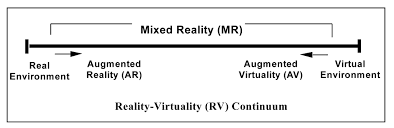
\includegraphics[width=\linewidth]{mixedrealitycontinuum}
	\caption{Mixed Reality Continuum (Source: \cite{milgram1995augmented})}
	\label{fig:mixedrealitycontinuum}
\end{figure}

Augmented reality has been defined by \textcite{azuma1997survey} as having the following three characteristics: 

\begin{enumerate}
	\item Combines real and virtual 
	\item Is interactive in real time
	\item Is registered in three dimensions
\end{enumerate} 

Virtual reality has been gaining popularity in the consumer market in recent years. It is a specific type of mixed reality featuring entirely digital visuals and virtual environments. No clear distinctions are made between points in the continuum. One particular construct, augmented reality, has been gaining popularity over the years. Augmented reality refers to systems that feature predominantly real environments whose perception maybe augmented with information not readily available to the user (figure \ref{fig:augreal} for example, shows a map overlay on top of the camera view of a street). Further, some factors have been identified that help distinguish between different mixed reality systems: extent of world knowledge (whether the augmentation takes place in a modeled world or not), reproduction fidelity (quality of display of the real/virtual objects) and extent of presence metaphor (extent to which user feels they are present in the displayed scene themselves). A detailed description of mixed reality displays and differences in their characteristics can be found in \cite{milgram1995augmented}. 

\begin{figure}
	\centering
	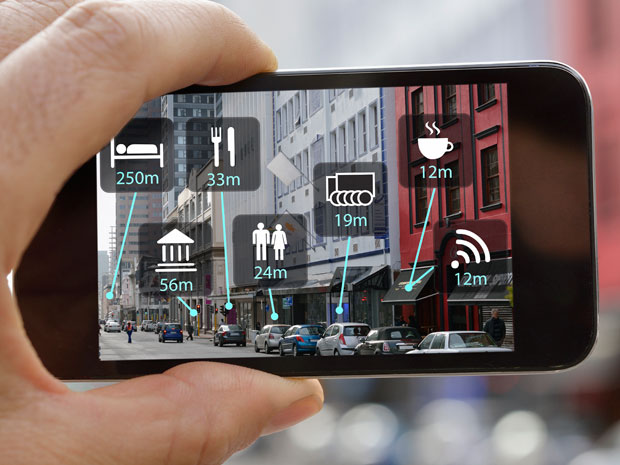
\includegraphics[width=\linewidth]{augreal}
	\caption{View of a street 'augmented' with information on places of interest}
	\label{fig:augreal}
\end{figure}
